% 导言区,进行全局设置
\documentclass[12pt]{ctexart}%book, report, latter, 引入文档类

%\usepackage{ctex}
%\usepackage[fleqn]{amsmath}
\usepackage{amsmath}
\usepackage{amssymb}
\usepackage{fancyhdr}
\usepackage{lastpage}
\usepackage{graphicx}
\usepackage{float}
\usepackage{enumerate} % when need define format to number by myself
\usepackage[colorlinks,linkcolor=black]{hyperref} % set super link

% \newcommand命令的定义,新的命令
\newcommand\degree{^\circ}
\title{\kaishu Ensemble Learning}
\author{Fish}
\date{\today}


% 内容与格式分离
% 设置标题的格式
\ctexset {
	section = {
		format+=\zihao {-4} \heiti \raggedright,
		name = {,},
		%number = \chinese{section},
		beforeskip = 1.0ex plus 0.2ex minus .2ex,
		afterskip = 1.0ex plus 0.2ex minus .2ex,
		aftername = \hspace{0pt}
	},
	subsection = {
		format+=\zihao{5} \heiti \raggedright,
		% name={\thesubsection},
		name = {,},
		%number = \arabic{subsection},
		beforeskip = 1.0ex plus 0.2ex minus .2ex,
		afterskip = 1.0ex plus 0.2ex minus .2ex,
		aftername = \hspace{0pt}
	}
}

% 正文区(文稿区),有且只有一个document环境
% \begim{*环境名称}
%        内容
% \end{*环境名称}
\begin{document}
	\maketitle
	%\clearpage
	\renewcommand{\contentsname}{Content} % set the 目录 to Content
	\tableofcontents
	\clearpage
	\pagestyle{fancy}
	\lhead{Ensemble Learning by wzs}                   
	\rhead{Page \thepage{} of \pageref{LastPage}}
	
	\section{\quad the relation between decision tree and random forest}
		\begin{enumerate}
			\item the decision treee of random forest take samplt independently each other .
			\item sample weighting :A
				\begin{figure}[H]
					\vspace{-0.2cm}  %调整图片与上文的垂直距离
					\setlength{\abovecaptionskip}{-0.2cm}   %调整图片标题与图距离
					%\setlength{\belowcaptionskip}{-1cm}   %调整图片标题与下文距离
					\centering
					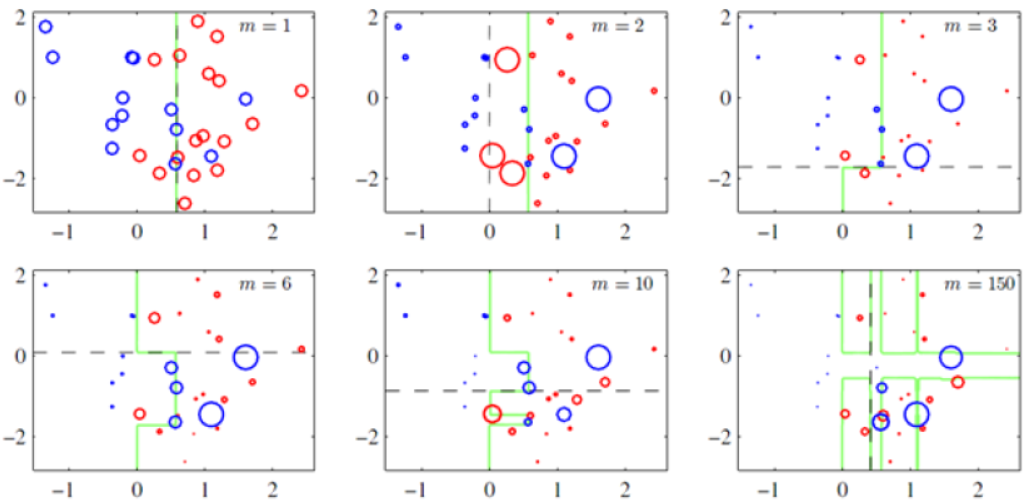
\includegraphics[scale=0.4]{sample_weighting.png}
					\renewcommand{\figurename}{Fig} % set picture title starting with Fig or 图
					\caption{samplt weighting}
					\label{fig:1}
				\end{figure}
		\end{enumerate}
	
	\section{\quad boosting}
		\subsection{\quad concept}
			\begin{enumerate}
				\item boosting is a technique, adapted to solve regression and classfication problem. it produce a weak predict model (like decision tree), and weghting cumulation to summary model, if the produce of weak model is depend on the gradient direction fo loss function every step, it is named gradient boostion.
				
				\item gradient boosting althgorithm make sure that a target loss function firstly, its definitin domain is the collection of weak function (basic fuction) all that are feasibility; it get be close to local minimal value choosing a basic function of negative gradient direction iteratly. this opinion about gradient boosting in function domain has a deep influence on machine learning.
				
				\item the meaning of boosting in theory:
				
				\qquad \qquad if a problem exit weak classifiter, then it could obtain strong classifiter by taking the method of boosting.
			\end{enumerate}
		
		\subsection{\quad boosting althgorithm}
			\begin{enumerate}
				\item form the any training sample $(x_1, y_1), (x_2, y_2), ..., (x_n, y_n)$ given the input vetor x and output variable y, the target is that find approximate functin $\hat{F}(\vec{x})$, make loss value of loss function $L(y, F(x))$ be least.
				
				\item typical definition of $L(y, F(x))$ is:
					\begin{align}
						L(y, F(\vec{x})) = \frac{1}{2}(y-F(\vec{x}))^2\\
						L(y, F(\vec{x})) = |y- F(\vec{x})|
					\end{align}
					
				\item assume that optimal function is $F^*(\vec{x})$, as follow:
					\begin{align}
						F^*(\vec{x}) =\mathop{\arg \min}\limits_F E_{(x,y)} \left[ L(y, F(\vec{x}))\right]
					\end{align}
					
				\item assume that $F(x)$ is the weghting sum of a collection of basic function $f_i(x)$
					\begin{align}
						F(\vec{x}) = \sum_{i=1}^{M}\gamma_i f_i(x) + const
					\end{align}
			\end{enumerate}
		
		\subsection{\quad derivation of boosting althgorithm}
			\begin{enumerate}
				\item find optimal solution $F(x)$ by gradient boostin althgorithm, let  the excetion fo loss function over the train set be least. the method as follow:
				
				\item firstly, given const function $F_0 (x)$ :
					\begin{align}
						F_0 (\vec{x}) = \mathop{\arg\min}\limits_\gamma \sum_{i=1}^{n}L(y_i, \gamma)
					\end{align}
					
				\item getting $F_m(x)$ by developing greedy thinking :
					 \begin{align}
					 	F_m(\vec{x}) = F_{m-1}(\vec{x}) + \mathop{\arg\min}\limits_{f\in H}\sum_{i=1}^{n}L(y_i, F_{m-1}(\vec{x}_i) + f(\vec{x}_i))
					 \end{align}
					 
				\item greedy method still is difficult when select optimal basic function every times.
					\begin{enumerate}
						\item to be approximate calculate using gradient descent method
						
						\item bring sample to basic function $f(x)$, get $f(x_1), f(x_2), ..., f(x_n)$, then L degrade into the vector $L(y_1, f(x_1))$, $L(y_2, f(x_2)), ..., L(y_n, f(x_n))$
							\begin{align}
								F_m(\vec{x}) = F_{m-1}(\vec{x}) - \gamma_m \sum_{i=1}^{n} \nabla_f L(y_i, F_{m-1}(\vec{x}_i))
							\end{align}

					\end{enumerate}
				
				\item among above equation, the weight value $\gamma$ is the step length of gradient descent, solve optimal step length using linear searching:
					\begin{align}
						\gamma_m = \mathop{\arg\min}_\gamma \sum_{i=1}^{n} L \left( y_i, F_{m-1}(\vec{x}_i) - \gamma\cdot\nabla_f L(y_i, F_{m-1}(\vec{x}_i) \right)
					\end{align}
			\end{enumerate}
			
		\subsection{\quad pseudo code of boosting algorithm }
			\begin{enumerate}
				\item given model be const initially: 
					\begin{align}
						F_0(\vec{x}) = \mathop{\arg\min}_\gamma \sum_{i=1}^{n} L(y_i, \gamma)
					\end{align}
					
				\item for $m=1$ to $M$:
					\begin{enumerate}
						\item calculate pseudo residuals: for $i = 1, 2, ..., n$
							\begin{align}
								r_{im} = \left[ \frac{\partial L(y_i, F(\vec{x}_i))}{\partial F(\vec{x}_i)}\right] _{F(\vec{x}) - F_{m-1}(\vec{x})}
							\end{align}
							
						\item calculate basic function $f_m(x)$ of fitting residuals using data $\{ (\vec{x}_i, r_{im})\} _{i=1}^n$
						
						\item calclulate step length 
							\begin{align}
								\gamma_m = \mathop{\arg\min}_\gamma \sum_{i=1}^{n} L \left( y_i, F_{m-1}(\vec{x}_i) - \gamma\cdot f_m(\vec{x}_i) \right)
							\end{align}
							\begin{itemize}
								\item optimal problem about one dimension
							\end{itemize}
							
						\item update model 
							\begin{align}
								F_m(\vec{x}) = F_{m-1}(\vec{x}) - \gamma _m f_m (\vec{x}_i)
							\end{align}
					\end{enumerate}
			\end{enumerate}
	
	\section{\quad gradient boosting decision tree GBDT}
		\subsection{\quad concept and algorithm theory}
			\begin{enumerate}
				\item the typical basic function of gradient boosting is decision tree (CART in particular)
				
				\item calculate decision tree $t_m(x)$ due to pseudo residuals data an mth gradient boosting. make the number of leaf node for tree $t_m(x)$ be J, then tree $t_m(x)$ devide the input space into J intersect area $R_{1m}, R_{2m}, ..., R_{Jm}$, and decision tree $t_m(x)$ could give assured prediction in every area. using indicated tag $I(x)$, for input x, $t_m(x)$ is:
					\begin{align}
						t_m(\vec{x}) = \sum_{j=1}^{J} b_{jm} I(\vec{x} \in R_{jm})
					\end{align} 
					
				\item among, $b_{jm}$ is the predict value that sample x in area $R_{jm}$
					
				\item minimize loss function using linear searching to calculate learning rate
					\begin{align}
						F_m(\vec{x}) &= F_{m-1}(\vec{x}) + \gamma\cdot t_m(\vec{x}_i)\\
						\gamma &= \mathop{\arg\min}_\gamma \sum_{i=1}^{n} L(y_i, F_{m-1}(\vec{x}_i) + \gamma\cdot t_m(\vec{x}_i))
					\end{align}
					
				\item what's more: calculate step length differentiatly for every area of tree, then combine the coefficient $b{jm}$ to step length. then :
					\begin{align}
						F_m(\vec{x}) &= F_{m-1}(\vec{x}) + \sum_{j=1}^{J}\gamma_{jm}I(\vec{x}\in{R_{jm}})\\
						\gamma_{jm} &= \mathop{\arg\min}_{\gamma} \sum_{\vec{x}_i\in{R_{jm}}} L(y_i, F_{m-1}(\vec{x}_i) + \gamma\cdot t_m(\vec{x}_i)) 
					\end{align}
			\end{enumerate}
	
		\subsection{\quad set parameter and regularization }
			\begin{enumerate}
				\item decline the generalization ability fitting training dataset over highly, need to regularization technique to decline over fitting.
					\begin{enumerate}
						\item increase penalty party for complex model, like: the complex degree is positive with leaf node number or the square fo predicted value of leaf node.
						
						\item be used to pruning of decision tree
					\end{enumerate}
				
				\item the number of leaf node control the number of layer of tree, select $4\leq J \leq 8$ in generally.
				
				\item leaf node contain least the number of sample
					\begin{enumerate}
						\item avoid occur over small leaf node, decline predicting variance.
					\end{enumerate}
				
				\item the number of iteration times M about gradient boosting
					\begin{enumerate}
						\item decline the loss value of training dataset by increase M, but exit the risk over fitting
						
						\item cross validation
					\end{enumerate} 
			\end{enumerate}
		
		\subsection{\quad summary of GBDT}
			\begin{enumerate}
				\item function estimate is treated as a problem in function space not parameter space originally. but phased additive expansion and gradient decline transfer function estimate into parameter estimate.
				
				\item loss function is least square error、 absolute error and so on, and is classfication problem; but error function is changed to more class Logistic likelihood function, and become a classification function.
				
				\item make target function divide into the weighted sum of any basic function, is common technique method: here could see its shaddow nenural network、 radial base function、 Fourier / wavelet transform、 SVM.
			\end{enumerate}
		
	\section{\quad XGBoost}
		\subsection{\quad sencond derivation information}
			\begin{enumerate}
				\item target function:
					\begin{align}
						J(f_t) = \sum_{i=1}^{n} L(y_i, \hat{y}_i^{(t-1)} + f_t(x_i)) + \Omega(f_t) + C
					\end{align}
					
				\item according to Taylor developing equation:
					\begin{align}
						f(x + \Delta x) \approx f(x) + f'(x)\Delta x + \frac{1}{2}f''(x)\Delta x^2
					\end{align}
					
				\item define,
					\begin{align}
						g_i \overset{def}{==} \frac{\partial L(y_i, \hat{y}_i^{(t-1)})}{\partial \hat{y}_i^{(t-1)}}\\
						h_i \overset{def}{==} \frac{\partial^2 L(y_i, \hat{y}_i^{(t-1)})}{\partial \hat{y}_i^{(t-1)}}
					\end{align}
				
				\item get:
					\begin{align}
						J(f_t) \approx \sum_{i=1}^{n} \left[ L(y_i, \hat{y}_i^{(t-1)}) + g_i f_t(x_i)) + \frac{1}{2} h_i f_t^2(x_i)\right] + \Omega(f_t) + C
					\end{align}
			\end{enumerate}
		
		\subsection{\quad describe of decision tree}
			\begin{enumerate}
				\item classfy or regress the sample using decision tree, the thining process from root node to leaf node, the predict value of sample that belong to alike leaf node is equal.
				
				\item assume that the number of leaf node of decision tree is T, weight value of every leaf node is $\vec{w} = (w_1, w_2, ..., w_T)$, the learning process of decision tree, also explain building process how to use feature devided and getting weight value.
				
				\item sample x is belong to leaf node q, define function : $f_t(x) = w_{q(x)}$
					\begin{itemize}
						\item the kernel of decision tree is "tree structure" and "leaf weight value"
					\end{itemize}
			\end{enumerate}	
		
		\subsection{\quad definition of regularization $\Omega(f_t)$}
			\begin{enumerate}
				\item the complex degree of decision depend on the number of leaf node and leaf weight value, like using weighting between the number of all leaf node and square sum of leaf weight value
					\begin{align}
						&\Omega(f_t) = \gamma \cdot T_t + \lambda \cdot \frac{1}{2}\sum_{j=1}^{T} w_j^2\\
						T: &\text{leaf number} \quad w_j^2: \text{square sum of weight} \notag
					\end{align}
			\end{enumerate}
			
		\subsection{\quad calculation and simplify of loss function}
			\begin{enumerate}
				\item calculation
					\begin{align}
						\begin{split}
							J(f_t) &\approx \sum_{i=1}^{n} \left[ L(y_i, \hat{y}_i^{(t-1)}) + g_i f_t(x_i)) + \frac{1}{2} h_i f_t^2(x_i)\right] + \Omega(f_t) + C\\
							&= \sum_{i=1}^{n} \left[ g_i f_t(x_i) + \frac{1}{2} h_i f_t^2(x_i)\right] + \Omega(f_t) + C\\
							&= \sum_{i=1}^{n} \left[ g_i w_{q(x_i)} + \frac{1}{2}h_t w_{q(x_i)}^2\right] + \gamma\cdot T + \lambda\cdot \frac{1}{2}\sum_{j=1}^{T}w_j^2 + C\\
							&= \sum_{j=1}^{T} \left[ \left( \sum_{i\in I_j}g_i \right) w_{j} + \frac{1}{2} \left( \sum_{i\in I_j}h_t \right)  w_{j}^2\right] + \gamma\cdot T + \lambda\cdot \frac{1}{2}\sum_{j=1}^{T}w_j^2 + C\\
							&= \sum_{j=1}^{T} \left[ \left( \sum_{i\in I_j}g_i \right) w_{j} + \frac{1}{2} \left( \sum_{i\in I_j}h_t + \lambda \right)  w_{j}^2\right] + \gamma\cdot T + C
						\end{split}
					\end{align}
					
				\item simplify target function
					\begin{enumerate}
						\item for : $J(f_t) = \sum\limits_{j=1}^{T} \left[ \left( \sum\limits_{i\in I_j}g_i \right) w_{j} + \frac{1}{2} \left( \sum\limits_{i\in I_j}h_t + \lambda \right)  w_{j}^2\right] + \gamma\cdot T + C$
						
						\item define $G_j \overset{def}{==} \sum\limits_{i\in I_j} g_i, \ H_j \overset{def}{==} \sum\limits_{i\in i_j} h_i$
						
						\item then, $J(f_t) = \sum\limits_{j=1}^{T} \left[ G_j w_{j} + \frac{1}{2} ( H_j + \lambda )  w_{j}^2\right] + \gamma\cdot T + C$
						
						\item derivate partially for w, getting
							\begin{align}
								\frac{\partial J(f_t)}{\partial w_j} &= G_j +(H_j + \lambda)w_j \overset{\text{令}}{==} 0\\
								\Rightarrow w_j &= -\frac{G_j}{H_j + \lambda}
							\end{align}
							
						\item bring back to target function, getting
							\begin{align}
								J(f_t) = -\frac{1}{2} \sum_{j=1}^{T} \frac{G_J^2}{H_j + \lambda} + \gamma \cdot T
							\end{align}
					\end{enumerate}
			\end{enumerate}
		
		\subsection{\quad example}
			\begin{enumerate}
				\item what
					\begin{figure}[H]
						\vspace{-0.2cm}  %调整图片与上文的垂直距离
						\setlength{\abovecaptionskip}{-0.2cm}   %调整图片标题与图距离
						%\setlength{\belowcaptionskip}{-1cm}   %调整图片标题与下文距离
						\centering
						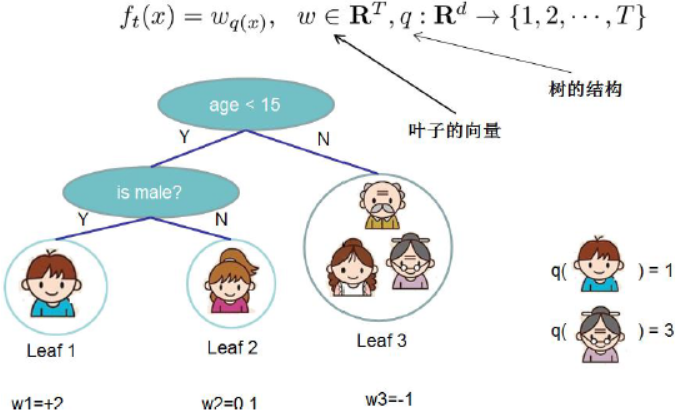
\includegraphics[scale=0.8]{XGBoost_example.png}
						\renewcommand{\figurename}{Fig} % set picture title starting with Fig or 图
						\caption{XGBoost example}
						\label{fig:2}
					\end{figure}
				
				\item penalty part
					\begin{align}
						\Omega = \gamma \cdot 3 + \frac{1}{2} \cdot \lambda \cdot (4 + 0.01 + 1)
					\end{align}
					
				\item calculation
					\begin{figure}[H]
						\vspace{-0.2cm}  %调整图片与上文的垂直距离
						\setlength{\abovecaptionskip}{-0.2cm}   %调整图片标题与图距离
						%\setlength{\belowcaptionskip}{-1cm}   %调整图片标题与下文距离
						\centering
						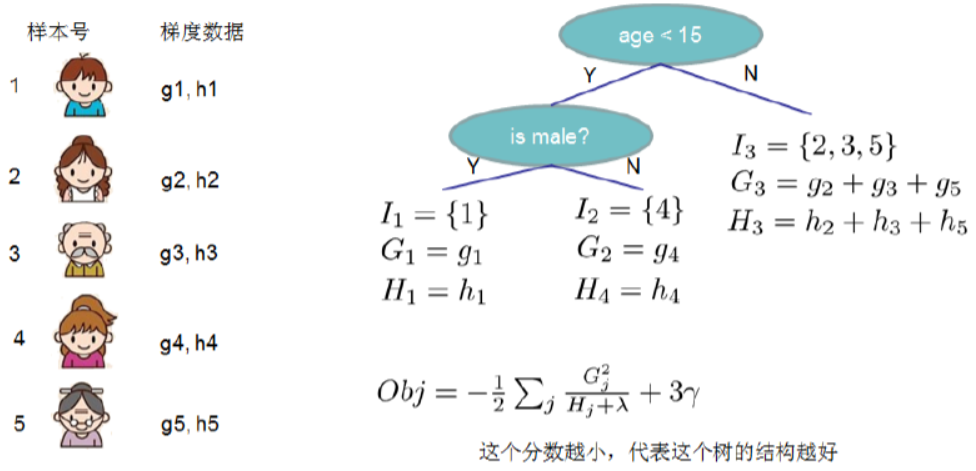
\includegraphics[scale=0.6]{XGBoost_example_calculation.png}
						\renewcommand{\figurename}{Fig} % set picture title starting with Fig or 图
						\caption{XGBoost example calculation}
						\label{fig:3}
					\end{figure}
				
				\item how to bulid the structure of decision tree $J(f_t) = -\frac{1}{2} \sum_{j=1}^{T} \frac{G_J^2}{H_j + \lambda} + \gamma \cdot T$
					\begin{enumerate}
						\item equestion: for current node, how to divide subtree?
						
						\item answer: use for reference the solution fo ID3/C4.5/CART, using greedy method:
							\begin{enumerate}
								\item for a feasible division, calculate the $j(f)$ after dividing
								
								\item for all feasible division, choose the segementation dot making $J(f)$ decline least
							\end{enumerate}
					\end{enumerate}
				
				\item enumerate feasible segemetation dot, select division of largest gain, continue same operation, until statify threshold or get pure node
					\begin{align}
						Gain(\phi) = \frac{1}{2} \left[ \frac{G_L^2}{H_L + \lambda} + \frac{G_R^2}{H_R + \lambda} - \frac{(G_L + G_R)^2}{H_L + H_R + \lambda} \right]
					\end{align}
					\begin{figure}[H]
						\vspace{-0.6cm}  %调整图片与上文的垂直距离
						\setlength{\abovecaptionskip}{-0.2cm}   %调整图片标题与图距离
						%\setlength{\belowcaptionskip}{-1cm}   %调整图片标题与下文距离
						\centering
						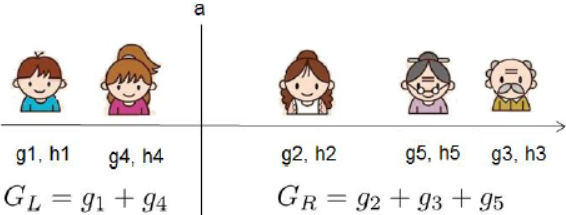
\includegraphics[scale=0.6]{XGBoost_example_calculation_result.png}
						\renewcommand{\figurename}{Fig} % set picture title starting with Fig or 图
						\caption{XGBoost example calculation result}
						\label{fig:4}
					\end{figure}
			\end{enumerate}
		
		
	\section{\quad Adaboosting}
		\subsection{\quad thinking}
			\begin{figure}[H]
				\vspace{-0.2cm}  %调整图片与上文的垂直距离
				\setlength{\abovecaptionskip}{-0.2cm}   %调整图片标题与图距离
				%\setlength{\belowcaptionskip}{-1cm}   %调整图片标题与下文距离
				\centering
				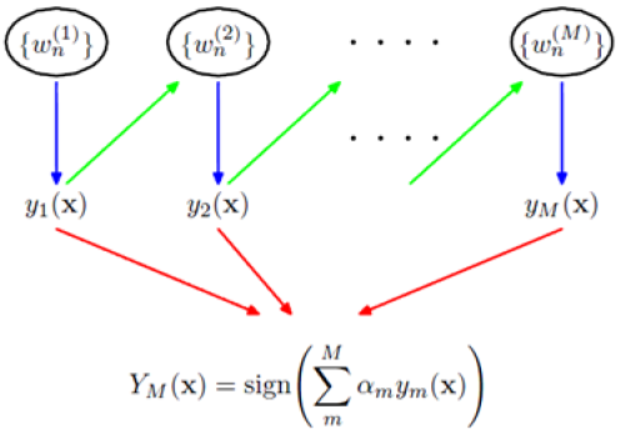
\includegraphics[scale=0.4]{boosting_thinking.png}
				\renewcommand{\figurename}{Fig} % set picture title starting with Fig or 图
				\caption{boosting thinking}
				\label{fig:5}
			\end{figure}
		
		\subsection{\quad algorithm}
			\begin{enumerate}
				\item assume training dataset $T = \{ (x_1, y_1), (x_2, y_2), ..., (x_N, y_N))\}$
				
				\item initialize the weight distribution of training dataset 
					\begin{align}
						D_1 = (w_{11}, w_{12}, ..., w_{1i}, ..., w_{1N}), \quad w_{1i} = \frac{1}{N}, \quad i=1,2,...,N
					\end{align}
					
				\item study algorithm using traning dataset that weight distribution is like $D_m$, get basic classfier
					\begin{align}
						G_m(x) : \chi \rightarrow \{ -1, +1\}
					\end{align}
					
				\item calculate the classfication error rate that $G_m(x)$ trained in training dataset
					\begin{align}
						e_m = P(G_m(x_i) \neq y_i) = \sum_{i=1}^{N} w_{mi} I(G_m(x_i) \ne y_i)
					\end{align}
					
				\item calculate the coefficient of $G_m(x)$
					\begin{align}
						\alpha_m = \frac{1}{2}\log{\frac{1-e_m}{e_m}}
					\end{align}
					
				\item update the weight distribution of training dataset
					\begin{align}
						D_{m+1} &= (w_{m+1, 1}, w_{m+1, 2}, ..., w_{m+1, t}, ..., w_{m+1, N})\\
						w_{m+1, i} &= \frac{w_{mi}}{Z_m} \text{exp} (-\alpha_m y_i G_m(x_i)), \quad i=1,2,..,N
					\end{align}
					
				\item here, $Z_m$ is standardization factor
					\begin{align}
						Z_m = \sum_{i=1}^{N} w_{mi} \text{exp} (-\alpha_m y_i G_m(x_i))
					\end{align}
					
					\begin{itemize}
						\item its purpose is only making $D_{m+1}$ become a probability distribution
							\begin{align}
								w_{m+1, i} &= \frac{w_{mi}}{Z_m} \text{exp} (-\alpha_m y_i G_m(x_i))\\
								\Rightarrow Z_m w_{m+1, i} &= w_{mi} \text{exp} (-\alpha_m y_i G_m(x_i))\\
								\Rightarrow Z_1 w_{2, i} &= w_{1i} \text{exp} (-\alpha_1 y_i G_1(x_i))
							\end{align}
					\end{itemize}
				
				\item build linear group of basic classfier
					\begin{align}
						f(x) = \sum_{m=1}^{M} \alpha_m G_m(x)
					\end{align}
					
				\item final classfier
					\begin{align}
						G(x) = sign(f(x)) = sign \left( \sum_{m=1}^{M} \alpha_m G_m(x) \right)
					\end{align}
			\end{enumerate}
\end{document}